\chapter{Optimización de Hiperparámetros}



\section{Planteo del Problema}

Sea $f: X \rightarrow \mathbb{R}$ una función que devuelve el máximo error de validación de un modelo entrenado a partir de una combinación de hiperparámetros $\textbf{x} \in X$, se desea encontrar $\hat{\textbf{x}}$:

\[
\textbf{x}^* = arg \min_{\textbf{x} \in X} f(\textbf{x})
\]

Es decir, se busca encontrar la combinación óptima de hiperparámetros dentro de un dominio $X$ para obtener el mínimo error de representación en un dado conjunto de validación. En el caso de la construcción de una base \textit{hp-greedy} óptima: 

\[
\textbf{x} = (n_{max}, l_{max}, \varepsilon, \hat{\Lambda}_0).
\]


%El hiperparámetro de mayor interés es sin duda la $semilla$, pues a primera vista no hay una forma obvia de elegir su valor óptimo. Además una semilla óptima para una combinación de $(n_{max_1}, l_{max_1})$ no lo será necesariamente para otra combinación $(n_{max_2}, l_{max_2})$.

%También se observó que en ciertas situaciones un valor muy elevado de $l_{max}$ o muy pequeño de la $tolerancia$ $greedy$ pueden conducir a un modelo \textit{sobreajustado}. Por esto es de interés realizar una optimización que involucre a la totalidad de los hiperparámetros dentro del dominio $X$. 

El problema al momento de realizar esta optimización es que la función $f$ no tiene una expresión analítica, sino es que es el resultado de entrenar el modelo y evaluar el error de representación con un conjunto de validación, lo que la hace costosa de evaluar (computacionalmente hablando). Este capítulo se centrará principalmente en la \textbf{optimización Bayesiana} \cite{7352306, https://doi.org/10.48550/arxiv.1012.2599}, un método que intenta reducir al mínimo el número de evaluaciones de $f$ para encontrar $\hat{\textbf{x}}$ y se puede colocar dentro de una categoría llamada optimización secuencial basada en modelos, o \textbf{SMBO}\cite{dewancker2015bayesian,NIPS2011_86e8f7ab} (\textit{Secuential Model-Based Optimization}).


Además existen dos métodos muy utilizados que no utilizan modelos, los cuales son la \textbf{búsqueda exhaustiva} (o \textit{grid search}) y la \textbf{búsqueda aleatoria}. Estos métodos se utilizaron en casos sencillos de optimización para realizar una comparación con la optimización bayesiana.


\subsubsection*{Comentario sobre el dominio $X$}


Si bien la tolerancia \textit{greedy} $\varepsilon$ puede tomar cualquier valor real no nulo (a diferencia de $n_{max}, l_{max}$ y $\hat{\Lambda}_0$ que toman valores discretos), para simplificar la búsqueda de $\hat{\textbf{x}}$ se utilizaron siempre distribuciones discretas en el espacio logarítmico. Más específicamente se utilizaron conjuntos de la forma $C = \{1\times 10^{t} \  | \ a \leq t \leq b,  t \in {\mathbb{Z}} \}$. De esta forma $X$ será un conjunto finito y estará definido por los valores extremos de cada hiperparámetro. 


\section{Optimización Bayesiana}

\begin{figure}[h!]
\centering
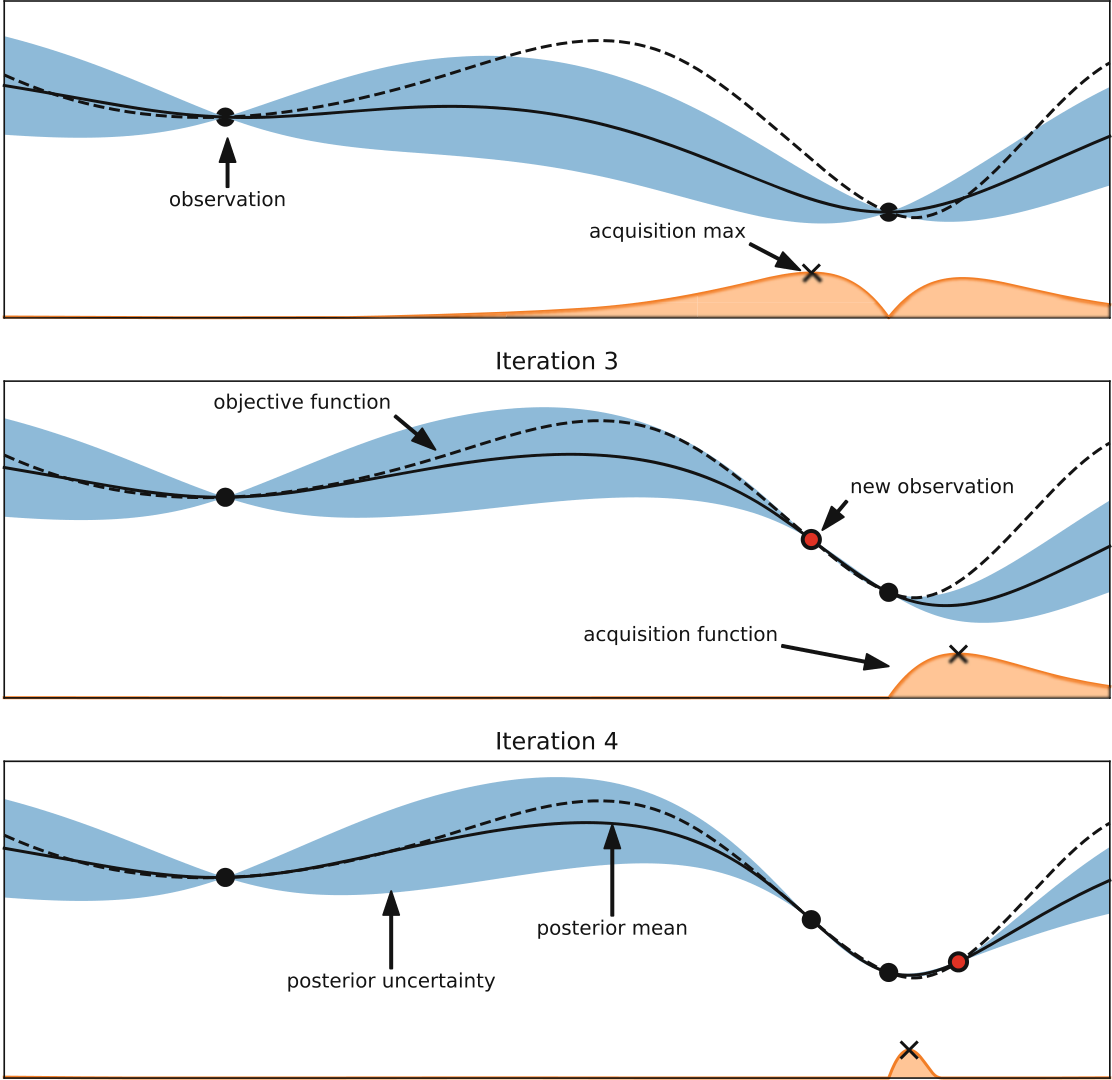
\includegraphics[width=.7\columnwidth]{bayesian.png}
\caption{En la figura se observan tres iteraciones de una optimización bayesiana para una función sencilla con parámetro unidimensional. En linea punteada está representada la función real, mientras que con linea gruesa se representa el valor medio del modelo estadístico (en este caso construido utilizando procesos gaussianos). El área pintada en azul representa la incertidumbre del modelo, que tiende a cero en los puntos que representan las observaciones realizadas. Debajo se puede ver una función de adquisición en color naranja, que indica el siguiente punto a evaluar \cite{Feurer2019}.}
\label{fig:bayesian}
\end{figure}

La optimización bayesiana es un método que utiliza la información de todas las evaluaciones realizadas de la función $f$ para decidir que valor de $\textbf{x}$ evaluar a continuación, reduciendo así el número necesario de evaluaciones de $f$ para encontrar el mínimo.

Para explicar como funciona este método se parte de un formalismo llamado optimización secuencial basada en modelos, que no es más que una generalización de la optimización bayesiana.

\subsection{Optimización Secuencial Basada en Modelos}

La idea es aproximar la función $f$ a partir de un modelo sustituto $\mathcal{M}$.

Se parte de un conjunto de observaciones $D = \{(\textbf{x}^{(1)},y^{(1)}), \cdots, (\textbf{x}^{(k)},y^{(k)}) \}$, donde $y^{(j)} = f(\textbf{x}^{(j)})$, a partir del cual se ajusta el modelo sustituto $\mathcal{M}$. Luego utilizando las predicciones del modelo se maximiza una función $S$ llamada función de adquisición que elije el siguiente conjunto de hiperparámetros $\textbf{x}_i \in X$ para evaluar la función $f$ y se agrega el par $(\textbf{x}_i, f(\textbf{x}_i))$ al conjunto de observaciones $D$. Una vez hecho esto se vuelve a ajustar el modelo $\mathcal{M}$ y se repite el proceso, que está explicado en forma de pseudocódigo en el algoritmo \ref{alg:SMBO}.

%En la optimización secuencial basada en modelos, cada evaluación de la función $f$ se decide en base a un conjunto $D$ de observaciones realizadas previamente. Esto se logra entrenando un modelo sustituto $\mathcal{M}$ en base al conjunto $D$, y luego utilizando una función $S$ llamada función de \textit{adquisición}, que decidirá el mejor punto a evaluar en la función real.

%Se parte de un conjunto $D = {(\textbf{x}}$ generado a partir de un muestreo de observaciones de la función $f$ de la forma $(\textbf{x}_j, f(\textbf{x}_j))$, a partir del cual se ajusta el modelo sustituto $\mathcal{M}$. Luego, maximizando la función de adquisición $S$ se elije el siguiente conjunto de hiperparámetros $\textbf{x}_i$ para evaluar la función $f$ y se agrega el par $(\textbf{x}_i, f(\textbf{x}_i))$ al conjunto de observaciones $D$. Una vez hecho esto se vuelve a ajustar el modelo $\mathcal{M}$ y se repite el proceso, que está explicado en forma de pseudocódigo en el algoritmo \ref{alg:SMBO}.


\begin{algorithm}
\caption{\texttt{SMBO}}
\label{alg:SMBO}
\begin{algorithmic}[1]
\Require $f, X, S,\mathcal{M}$
\State $D =$ InicializarMuestras$(f, X)$
\vspace{1mm}
\For{$i = 1, 2, ...$}
	\State $\mathcal{M} =$ AjustarModelo$(D)$
	\State $\textbf{x}_{i} = arg \max_{\textbf{x}\in X} \mathcal{S}(\textbf{x}, \mathcal{M})$ .
	\State $y_i = f(\textbf{x}_i)$	\Comment{Paso costoso}
	\State $D = D \cup \{(\textbf{x}_i, y_i)\}$
\EndFor
\vspace{3mm}

\end{algorithmic}
\end{algorithm}

\subsection*{Optimización Bayesiana}

Lo que caracteriza a la optimización bayesiana dentro del formalismo de la optimización secuencial basada en modelos, es justamente la creación del modelo.
En la optimización bayesiana se construye un modelo estadístico, donde se representa con  $P(y|\textbf{x})$ la predicción del modelo, siendo $y$ el resultado de una evaluación $f(\textbf{x})$. El nombre del método se debe a que para la construcción del modelo se utiliza el teorema de Bayes:
  
 \[
 P(y|\textbf{x}) = \frac{P(\textbf{x}|y) \ P(y)}{P(\textbf{x})}
 \]
 
En la terminología bayesiana, se conoce a $P(y|\textbf{x})$ como probabilidad a posteriorí o \textit{posterior}, que es proporcional a la probabilidad a priori o \textit{prior} $P(y)$ por la función de verosimilitud o \textit{likelihood} $P(\textbf{x}|y)$. La probabilidad $P(\textbf{x})$ es una probabilidad marginal que sirve como factor de normalización, por lo que no es de tanto interés.


\subsubsection*{Procesos Gaussianos}

\begin{figure}[h!]
\centering
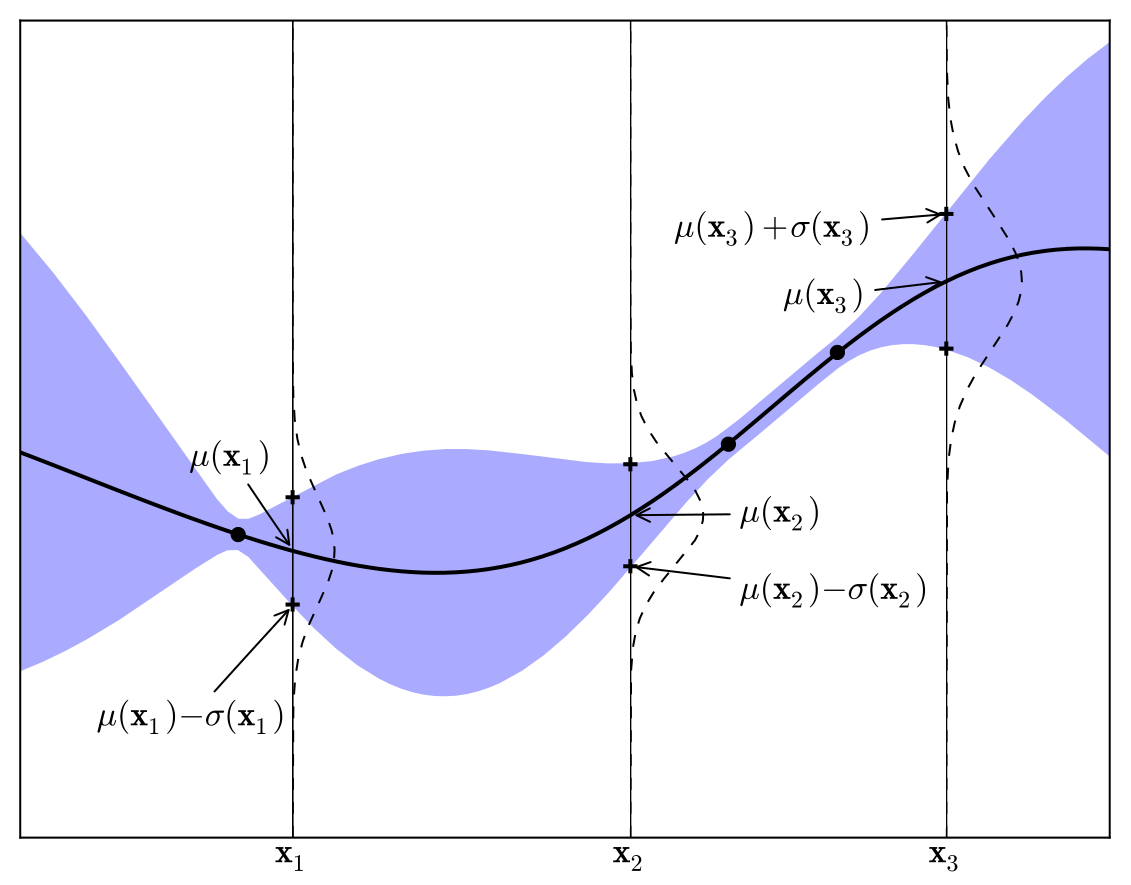
\includegraphics[width=.8\columnwidth]{gaussian.png}
\caption{Proceso Gaussiano unidimensional con tres observaciones representadas por los puntos negros. La linea gruesa representa la media del modelo predictivo y la zona azul la varianza en cada caso. Se representa con linea de trazo las distribuciones normales para los valores $x_1, x_2,$ y $x_3$\cite{https://doi.org/10.48550/arxiv.1012.2599}.}
\label{fig:gaussian}
\end{figure}

Una opción muy utilizada para la construcción del \textit{prior} y actualización del \textit{posterior} son los procesos gaussianos. Una forma sencilla de entender un proceso gaussiano es pensarlo como una función que para cada valor de $x$ devuelve la media $\mu(x)$ y la varianza $\sigma(x)$ de una distribución normal, en el caso particular de que $x$ sea unidimensional (ver figura \ref{fig:gaussian}). Con $\textbf{x}$ multidimensional, se obtiene una distribución normal multivariante, caracterizada por el vector $\bm{\mu}(\textbf{x})$ y la matriz de covarianza $\Sigma(\textbf{x}, \textbf{x}')$.

Sin embargo en este trabajo no se utilizan procesos gaussianos, principalmente porque parten del supuesto de que $f$ es continua. En su lugar se utiliza el estimador de Parzen con estructura arbórea, que se explicará en la sección \ref{sec:TPE}.

Para una introducción a la optimización bayesiana con procesos gaussianos ver \cite{https://doi.org/10.48550/arxiv.1012.2599}.

\subsection{Mejora Esperada: Función De Adquisición} 
 
%Debido a que la función $f$ no será necesariamente convexa, y seguramente tendrá varios mínimos locales, es necesario mantener un equilibrio entre la explotación y la exploración, es decir, explorar los mínimos tentativos sin dejar de lado las zonas inexploradas, en donde podría haber algún mínimo por descubrir. De esto se encarga la función de adquisición.
Para la elección de los puntos a evaluar en la función real se maximiza la función de adquisición $S$. Existen varias propuestas de funciones de adquisición, pero en este caso se utiliza la \textbf{mejora esperada} o \textit{Expected Improvement} (EI) \cite{EI1}. Sea $y^*$ un valor de referencia, se define a la mejora esperada  con respecto a $y^*$ como:


\begin{equation}
\label{eq:ei_def}
EI_{y^*}(\textbf{x}) := \int_{-\infty}^{\infty} \max(y^*-y,0) p(y|\textbf{x}) \ dy
\end{equation}
 

\subsection{Estimador de Parzen con Estructura Arbórea} 
\label{sec:TPE}

 El estimador de Parzen con estructura arbórea o \textbf{TPE} (\textit{Tree-Structured Parzen Estimator}) \cite{NIPS2011_86e8f7ab} es una estrategia que modela $P(x_i|y)$ para cada $x_i \in X_i$ (es decir, que $x_i$ representa a cada hiperparámetro por separado) a partir de dos distribuciones creadas a utilizando las observaciones $D$:

\begin{equation}
\label{eq:tpe}
P(x_i|y) =
	\begin{cases}
		\ell (x_i) & \text{si } y <y^{*} \\
		g(x_i) & \text{si } y \geq y^{*},
	\end{cases}
\end{equation}


Donde las densidades $\ell(x_i)$ y $g(x_i)$ se construyen a partir de dos conjuntos $D_{\ell}$ y $D_g$, ambos subconjuntos de $D$, tal que $D_{\ell}$ contiene todas las observaciones con $y < y^*$, y $D_g$ contiene a todo el resto de forma que $D = D_{\ell} + D_g$. El valor de referencia $y^{*}$ será un valor por encima del mejor valor observado de $f(\textbf{x})$, que se selecciona para ser un cuantil $\gamma \in (0,1)$ de los valores observados $y$ tal que $P(y<y^{*}) = \gamma$.


\subsubsection*{Mejora Esperada con TPE}
Aplicando la ecuación \eqref{eq:tpe} a la definición de mejora esperada \eqref{eq:ei_def} se obtiene la siguiente relación \cite{NIPS2011_86e8f7ab}:

\begin{equation}
EI_{y^*}(x_i) \propto \left( \gamma + (1-\gamma) \frac{g(x_i)}{\ell (x_i)} \right)^{-1}
\end{equation}

Es decir que para maximizar la mejora esperada se debe escoger un valor $x_i$ que maximice el cociente $\ell(x_i)/g(x_i)$ (o minimice $g(x_i)/\ell(x_i)$).

\subsubsection*{Estimación de las Densidades}

Las densidades de probabilidad se estiman utilizando ventanas de Parzen. Sea $D_x = \{x_i \ | \ (\textbf{x}, y) \in D_{\ell} \ (o\ D_g) \}$:

\begin{equation}
P(x_i) = \frac{\sum_{x_i'\in D_x}w_{x_i'}k(x_i, x_i') + w_p k(x_i, x_p) }{\sum_{x_i'\in D_x}w_{x_i'}+w_p},
\end{equation}
 

donde $w_{x_i'}$ es el peso de la observación $x_i'$, $x_p$ es un valor fijo \textit{prior}, $w_p$ es un peso \textit{prior} y $k$ es la función \textit{kernel}, que en este caso son distribuciones gaussianas truncadas $\mathcal{N}_{trunc}(\mu, \sigma, a, b)$ centradas en los puntos $x_i'$ (es decir, $\mu = x_i´$) con $a$ y $b$ límites inferior y superior del dominio. Por defecto los pesos $w_{x_i'}$ y $w_p$ son iguales a $1$. Para ver más detalles ver \cite{10.1613/jair.1.13188} y \cite{NIPS2011_86e8f7ab}.

%LEER https://tech.preferred.jp/en/blog/multivariate-tpe-makes-optuna-even-more-powerful/ !!!

\subsection*{Algoritmo}

Finalmente se puede ver el procedimiento completo del estimador de Parzen con estructura arbórea en el algoritmo \ref{alg:TPE}. Un detalle importante es que el algoritmo requiere un valor $n_c$, que es el número de candidatos que se utilizarán para maximizar el cociente $\ell(x_i)/g(x_i)$ (es decir, para maximizar la función de adquisición). En la linea 6 del algoritmo se realiza el muestro de los $n_c$ candidatos, utilizando la distribución $\ell(x_i)$, para luego seleccionar $x_i^*$ a partir del conjunto $C_i$.
Para este trabajo se utilizó la implementación de este algoritmo realizada en el paquete \textbf{\textit{Optuna}} \cite{optuna_2019} escrito en el lenguaje de programación Python.

\begin{algorithm}
\caption{\texttt{TPE}}
\label{alg:TPE}
\begin{algorithmic}[1]
\Require
\begin{tabular}{c}
$D = \{(\textbf{x}^{(1)},y^{(1)}), \cdots, (\textbf{x}^{(k)},y^{(k)}) \}$ \Comment{Observaciones}  \\ 
$n_t \in \mathbb{N}$ \Comment{número de iteraciones} \\ 
$n_c \in \mathbb{N}$ \Comment{número de candidatos} \\
$\gamma \in (0,1) $ \Comment{cuantil para obtener $y^*$}
\end{tabular} 

\vspace{1mm}
\For{$t = 1, 2, ..., n_t$}
	\State $D_{\ell} = \{ (\textbf{x}, y) \in D | y < y^*, \ \text{con } P(y<y^*) = \gamma  \}$
	\State $D_g = D - D_{\ell}$
	\For{$x_i = n_{max}, l_{max}, \varepsilon ,...$} \Comment{Para cada hiperparámetro}
		\State Construir $\ell(x_i)$ con $\{x_i \ | \ (\textbf{x}, y) \in D_{\ell}\}$ y $g(x_i)$ con $\{x_i \ | \ (\textbf{x}, y) \in D_g \}$.
		\State $C_i = \{ x_i^{(j)} \sim \ell(x_i)| j=1, ..., n_c \}$ \Comment{muestreo de $n_c$ candidatos para $x_i^*$}
		\State $x_{i}^* = arg \max_{x_i\in C_i} \ell(x_i)/g(x_i)$
	\EndFor
	\State $D = D \cup \{(\textbf{x}^*, f(\textbf{x}^*)\}$ \Comment{$\textbf{x}^*$ es el vector construido a partir de cada $x_i$.}
\EndFor
\Ensure $\textbf{x}$ con el mínimo valor $y$ en $D$.
\vspace{3mm}

\end{algorithmic}
\end{algorithm}
 
\subsection*{Paralelización}
 
El algoritmo escrito en Optuna permite paralelizar el proceso de optimización de forma asincrónica; esto se logra utilizando un método llamado \textit{mentiroso constante} (\textit{constant liar}) \cite{NIPS2011_86e8f7ab}. Consiste en que al proponer un valor $\textbf{x}^*$ se asigne temporalmente una evaluación falsa igual al promedio de los valores de $y$ medidos, que luego se actualizará al valor obtenido al momento de finalizar la evaluación real. Este proceso puede hacer la optimización menos eficiente con respecto al número de iteraciones, pero más rápida a fin de cuentas ya que se pueden realizar varias iteraciones a la vez.
 
\subsubsection*{TPE Multivariante} 

Una alternativa al algoritmo \ref{alg:TPE} es el algoritmo \textbf{TPE Multivariante}, implementado en Optuna \footnote{El algoritmo TPE Multivariante fue introducido en la siguiente actualización de Optuna: \url{https://github.com/optuna/optuna/pull/1767}}. La única diferencia es que en este caso las densidades no se construyen para cada hiperparámetro por separado, sino que se utilizan ventanas de Parzen multivariadas, dónde las funciones \textit{kernel} ahora son distribuciones gaussianas multivariadas. Es decir que en lugar de construir $\ell(x_i)$ y $g(x_i)$ para cada hiperparámetro, ahora se construye directamente $\ell(\textbf{x})$ y $g(\textbf{x})$.


\section{Optimización Multiobjetivo}

En este sección se explicará de forma básica el funcionamiento del algoritmo MOTPE (\textit{Multiobjective Tree-Structured Parzen Estimator}) \cite{10.1613/jair.1.13188, 10.1145/3377930.3389817}.%, sin entrar en demasiados detalles, pues si bien es un método interesante, se puede conseguir un mejor resultado utilizando el TPE clásico, y limitando el máximo valor de $n_{max}$ permitido. 

\subsection{Planteo del Problema}

Minimizar el error de representación no es el único objetivo posible al momento de construir una base reducida \textit{hp greedy}. También es de mucho interés minimizar el tiempo necesario para proyectar un conjunto de validación más denso a la base ya creada. Esto se debe a que se espera que un menor tiempo de proyección de lugar a un modelo más rápido de evaluar, que es el objetivo planteado a largo plazo.


Esta optimización se puede plantear como el problema de minimizar la función $\textbf{f}(\textbf{x})$:
\[
 \min_{\textbf{x} \in X} \textbf{f}(\textbf{x}) := (f_1(\textbf{x}), f_2(\textbf{x}))
\]

Cuando se quiere minimizar dos o más objetivos a la vez aparece el problema de que estos entran en conflicto entre sí, por lo que ya no se puede hablar de encontrar un valor mínimo en general, pero sí se puede encontrar un conjunto de elementos llamado \textbf{frente de Pareto} formado por los mejores valores encontrados. Con el conjunto de Pareto se decidirá que objetivo es más importante relativo al resto, y se elegirá el valor deseado.

Para entender mejor esto y el algoritmo MOTPE se empezará con algunas definiciones matemáticas que serán relevantes.

\subsection{Preliminares Matemáticos}

\noindent\textbf{Definición 1} Relación de Dominancia. Un vector $\textbf{y} \in \mathbb{R}^n$ domina al vector $\textbf{y'} \in \mathbb{R}^n$ si y solo si $\forall i: y_i \leq y_i'$ y $\exists i : y_i < y_i'$, y se denota con $\textbf{y} \prec \textbf{y'} $. Un vector $\textbf{y} \in \mathbb{R}^n$ domina débilmente al vector $\textbf{y'} \in \mathbb{R}^n$ si y solo si $\forall i: y_i \leq y_i'$, y se denota con $\textbf{y} \preceq \textbf{y'} $. \\


\noindent\textbf{Definición 2} Relación incomparable. Dos vectores $\textbf{y},\textbf{y'} \in \mathbb{R}^n$ son incomparables si y solo si no se cumple que $\textbf{y} \preceq \textbf{y'} $ ni que $\textbf{y'} \preceq \textbf{y} $, y se denotan $\textbf{y}||\textbf{y'}$.\\


%\noindent\textbf{Definición 3} Rango no dominante. Para un conjunto finito de vectores $Y \subset \mathbb{R}^n$, el rango no dominante de un vector $\textbf{y} \in Y$, denotado $rango(\textbf{y}) \in \mathbb{N}$ se define de la siguiente manera:

%\begin{itemize}
%\item rango$(\textbf{y}) = 1$, sii $\nexists \ \textbf{y'} \in Y : \textbf{y'} \prec \textbf{y}.$
%\item rango$(\textbf{y}) = \max_{\textbf{y'} \in Y'}\text{rango}(\textbf{y'}) + 1, \text{ donde } Y' = \{ \textbf{y'} \in Y | \textbf{y'} \prec \textbf{y}\}.$
%\end{itemize}
%Un vector $\textbf{y} \in Y$ no está dominado sii rango$(\textbf{y})=1$. Se denota con $ Y_{rango(k)}$ al conjunto $\{ \textbf{y} \in Y | \text{rango}(\textbf{y}) = k \}$.\\


\noindent\textbf{Definición 3} Relación de dominancia entre un vector y un conjunto. Para un conjunto finito de vectores $Y \subset \mathbb{R}^n$ y un vector $\textbf{y} \in \mathbb{R}^n$, se define $Y \prec \textbf{y}$ ($Y \preceq \textbf{y}$) si y solo si $\exists \ \textbf{y'} \in  Y_{rango(1)}:\textbf{y'} \prec \textbf{y}$ ($\textbf{y'} \preceq \textbf{y}$). También se define $\textbf{y} \prec Y$ ($\textbf{y} \preceq Y $) si y solo si $\exists \ \textbf{y'} \in  Y_{rango(1)}:\textbf{y} \prec \textbf{y'}$ ($\textbf{y} \preceq \textbf{y'}$).\\


\noindent\textbf{Definición 4} Relación Incomparable entre un vector y un conjunto.  Para un conjunto finito de vectores $Y \subset \mathbb{R}^n$ y un vector $\textbf{y} \in \mathbb{R}^n$, se define que $Y || \textbf{y}$ (equivalente a $\textbf{y}||Y$) si y solo si $\forall \textbf{y'}\in Y_{rango(1)}:\textbf{y}||\textbf{y'}$.\\


\noindent \textbf{Definición 5} Óptimo de Pareto. Dada una función $\textbf{f}: X \rightarrow \mathbb{R}^n$, un vector $\textbf{x}\in X$ es óptimo de Pareto si y solo si $\nexists \textbf{x'}\in X: \textbf{f(x')} \prec \textbf{f(x)} $. Un conjunto de vectores óptimos de Pareto $\{ \textbf{x} \in X | \nexists \textbf{x'}\in X: \textbf{f(x')} \prec \textbf{f(x)} \}$ se llama conjunto de Pareto. El conjunto de las imágenes del conjunto de Pareto $\{ \textbf{f(x)} \in \mathbb{R}^n | \textbf{x}\in X \text{es óptimo de Pareto} \}$ se llama frente de Pareto.


%\noindent \textbf{Definición 7} Indicador de hipervolumen. Sea $\lambda(S)$ la medida de Lebesgue (que en $\mathbb{R}^2$ coincide con una medida de área) de un conjunto medible $S$, el indicador de hipervolumen $I_H$ de un conjunto finito de vectores $Y \subset \mathbb{R}^n$ con un punto de referencia $\textbf{r} \in \mathbb{R}^n$ se define como:

%\begin{equation}
%I_H(Y; r) := \lambda(\{ \textbf{y} \in \mathbb{R}^n| Y \preceq \textbf{y} \preceq \textbf{r} \})
%\end{equation}

%En adelante se expresará como $I_H(Y)$, omitiendo el $\textbf{r}$ cuando su elección no sea relevante.

%\noindent \textbf{Definición 8} Contribución al hipervolumen. Para un conjunto finito de vectores $Y \subset \mathbb{R}^n$ y un vector $\textbf{y} \in Y$, la contribución de $\textbf{y}$ a $Y$ se define como $I_H(Y) - I_H(Y - \{ \textbf{y} \}).$

Lo más importante de esta subsección es entender la relación de dominancia y el concepto del frente de Pareto.

\subsection{Estimador de Parzen Multiobjetivo con Estructura Arbórea}

El MOTPE es una extensión del TPE clásico, adaptado para optimizar una función multiobjetivo.

Dado el conjunto de observaciones $D = \{(\textbf{x}^{(1)},\textbf{y}^{(1)}), \cdots, (\textbf{x}^{(k)},\textbf{y}^{(k)}) \}$, donde $\textbf{y}^{(j)} = \textbf{f}(\textbf{x}^{(j)})$, se modela $P(x_i|\textbf{y})$ para cada hiperparámetro $x_i$ usando las funciones de densidad de probabilidad $\ell(x_i)$ y $g(x_i)$:


\begin{equation}
\label{eq:motpe}
P(x_i|\textbf{y}) =
	\begin{cases}
		\ell (x_i) & \text{si } (\textbf{y} \prec Y^*) \vee (\textbf{y} \| Y^*) \\
		g(x_i) & \text{si } Y* \preceq \textbf{y},
	\end{cases}
\end{equation}

con $Y^*$ un conjunto construido tal que $p((\textbf{y} \prec Y^*) \vee (\textbf{y} \| Y^*)) = \gamma$. Nuevamente, $\gamma \in (0,1)$ es un cuantil, y las funciones $\ell(x_i)$ y $g(x_i)$ se construyen utilizando ventanas de Parzen en base a las observaciones realizadas.

En este caso la función de \textbf{mejora esperada} es un poco más complicada, pero se reduce al mismo resultado que con el TPE clásico; para maximizar la mejora esperada se debe maximizar la relación $\ell(x_i)/g(x_i)$ para cada $x_i$. Para ver en mayor detalle este resultado y el algoritmo completo del método, se recomienda ver \cite{10.1613/jair.1.13188}.





